%======================= CROSS-MEDIA IMAGE RETRIEVAL ===========================

\graphicspath{{img/t2v/}}

\def\t{\mathbf{t}} % t
\def\s{\mathbf{s}} % s
\def\e{\mathbf{e}} % e
\def\E{\mathbf{E}} % E

\newcommand{\ttv}{\textsc{Text2Vis}}
\newcommand{\sparsettv}{\textsc{S-Text2Vis}}
\newcommand{\densettv}{\textsc{D-Text2Vis}}
\newcommand{\widedeepttv}{\textsc{W\&D-Text2Vis}}
\newcommand{\visreg}{\textsc{VisReg}}
\newcommand{\wordvisual}{\textsc{Word2VisualVec}}
\newcommand{\resnet}{\gls{resnet}-152}

\chapter{\gls{cnn} Features Prediction for Cross-media Image Retrieval}
\label{ch:text2vis}

%%% ABSTRACT
% In this paper we tackle the problem of image search when the query is a short textual description of the image the user is looking for.
%We choose to implement the actual search process as a similarity search in a visual feature space, by learning to translate a textual query into a visual representation.
%Searching in the visual feature space has the advantage that any update to the translation model does not require to reprocess the (typically huge) image collection on which the search is performed.
%We propose various neural network models of increasing complexity that learn to generate, from a short descriptive text, a high level visual representation in a visual feature space such as the pool5 layer of the \resnet{} or the fc6-fc7 layers of an AlexNet trained on ILSVRC12 and Places databases.
%The \ttv{} models we explore include (i) a relatively simple regressor network relying on a \acrlong{bow} representation for the textual descriptors, (ii) a deep recurrent network that is sensible to word order, and (iii) a wide and deep model that combines a stacked LSTM deep network with a wide regressor network.
%We compare the models we propose with other search strategies, also including textual search methods that exploit state-of-the-art caption generation models to index the image collection.

Using a textual query to retrieve images is a very common cross-media search task, as text is the most efficient media to describe the kind of image the user is searching for.
Each media has its own representation space, which is modeled on a collection of representative content for that media.
For example, text can be represented by means of a simple \acrlong{bow} feature space, with the feature space being defined by a dictionary of observed words; or by means of more complex distributional semantic models, such as those based on neural networks, e.g., Word2Vec \cite{mikolov2013distributed}.
Similarly, a visual space can be modeled by identifying a set of relevant visual features in a collection on images, e.g., as those extracted by the deeper layers of \acrfullpl{cnn} \cite{krizhevsky2012imagenet}.
%\todo{Espandere sul visual space?}

In cross-media retrieval, the actual retrieval process can be implemented in a number of ways, depending on how the two feature spaces are joined.
The cross-media search space can be i) a textual feature space, i.e.,  a space whose definition is determined exclusively by observing textual content, ii)
a visual feature space, i.e.,  a space whose definition is determined exclusively by observing visual content,
or iii) a common latent space in which textual and visual features are projected into.

Using textual features is the most common solution. %, specially at the Web scale.
Each image is associated with a set of textual features extracted from its context of use --- e.g., the text surrounding the image in the Web page, description fields in metadata --- and eventually enriched by means of classifiers that assign textual labels related to the presence of certain relevant entities or abstract properties in the image.
The textual search space model can exploit the actual visual content of the image only when classifiers for the concepts of interest are available, thus requiring a relevant number of classifiers.
This also requires to reprocess the entire image collection whenever a new classifier is made available.

Searching in a common latent space requires learning two projections, i.e.,  from text-to-latent and from image-to-latent.
The main advantage of searching in a common latent space lies on the freedom the system has to jointly model reciprocal relations between the two media, while other strategies can only learn the relations from the source media to the target media, but not vice versa.
However, as in the textual space, projecting into a common latent space also requires to reprocess all the images whenever the textual model is updated, since the latent space where images are projected into is also influenced by the textual model part.
It also requires managing and storing the additional latent representations that are used only for the cross-media search.

A last, less explored, possibility is to use a visual space to convert any textual query into a visual representation.
A key advantage of this model is that the representation of images remains unaltered regardless of the projection model being developed.
This means that any improvement in the projection model --- e.g., in the underlying language model --- has immediate effects on the image retrieval process without requiring to reprocess the (typically huge) whole image collection and to rebuild the similarity search data structures required for efficient retrieval.
Another advantage is that --- since the visual space is language-independent --- multiple models, e.g., for multiple languages or specialized on different domains, can be used independently on the same collection of images, without requiring multiple instances of representations for the images and multiple instances of similarity search data structures.

In this chapter, we explore the use of a visual space for cross-media retrieval.
Methods that use a common space projection may be able to produce better results because they can exploit cross-correlations between the two media, while the other two approaches are constrained to leverage on correlations that come from one single direction.
However, we deem that the ability of using a single static collection of visual representations for images --- irrespectively to how many text-to-visual projection models are used and how often they change --- is a practical advantage of visual space-based methods that counters such possible loss of quality in results.

We present %the preliminary results on learning
\ttv{}, a family of neural network models that convert textual descriptions into visual representations in the same space of those extracted from \glspl{dcnn} such as the AlexNet~\cite{krizhevsky2012imagenet} or \resnet{}~\cite{he2016deep} trained on \gls{ilsvrc}'12~\cite{russakovsky2015imagenet} and Places~\cite{zhou2014learning} datasets.
% We first offer an overview of relevant cross-media retrieval in \ref{sec:t2v:related}.
We propose different neural network models of increasing complexity in \ref{sec:t2v:method}, including i) \sparsettv{}, a simple regressor network relying on sparse representations (bag-of-words and bag-of-bigrams) for the textual descriptors; ii) \densettv{}, a deep recurrent network relying on a continuous dense representations (word embeddings); and iii) \widedeepttv{}, a wide and deep architecture relying on both sparse and dense representations.
We report experimental results in \ref{sec:t2v:experiments}, comparing with other methods that use different projection approaches.
\ref{sec:t2v:conclusions} concludes and outlines possible directions for future research.

%---------------------------------------------------------------------
\section{Generating Visual Representations of Text}
\label{sec:t2v:method}

Our goal is to map textual descriptions to high-level visual representations.
As the visual space, we used the \emph{pool5} layer of the \resnet{} ~\cite{he2016deep} trained on \gls{ilsvrc}'12, and the \emph{fc6} and \emph{fc7} layers of the HybridNet~\cite{zhou2014learning} (i.e., an AlexNet ~\cite{krizhevsky2012imagenet} trained on both \gls{ilsvrc}'12 and Places datasets).
\acrfull{pca} and whitening are commonly used in retrieval processes based on vector similarity to reduce the dimensionality and to improve the retrieval effectiveness of visual features.
Projecting the dataset onto the eigenvectors results in no correlation between the components, while
whitening normalizes the vectors to have unit variance for all components.
This is done by simply dividing each component by the square root of its eigenvalue.
Originally proposed for local features aggregations such as \gls{vlad}~\cite{jegou2012negative}, \gls{pca} and whitening are also largely used for processing the activation of neurons \cite{sharif2014cnn,gong2014multi,gordo2016deep}.
As reported in \ref{subsec:t2v:results}, we observed relevant improvement by applying \gls{pca} and whitening to the visual features.

In this section, we describe the experimental activities we have carried out in order to achieve our goal.
We take a simple feed-forward regressor as a starting point (\ref{subsec:t2v:vis-reg}) to then propose three different architectures of increasing complexity: a regressor learning from unordered sparse features, called \sparsettv{} (\ref{subsec:t2v:sparse-t2v}); a deep recurrent network learning from ordered dense features, called \densettv{} (\ref{subsec:t2v:dense-t2v}); and a wide \& deep neural network which jointly learns from both types of representations, called \widedeepttv{} (\ref{subsec:t2v:wd-ttv}).

%------------------------------------------

\subsection{\visreg{}}
\label{subsec:t2v:vis-reg}

As a reference baseline, we started with a simple feed-forward regressor model with a hidden layer trained on the sparse one-hot representation of the textual input to directly predict the visual representation of the image (\ref{fig:t2v:visreg:arch}).
We observed a strong tendency to overfit (\ref{fig:t2v:visreg:loss}), thus degrading the applicability of the method to unseen images.

\begin{figure}
\begin{subfigure}{0.37\textwidth}
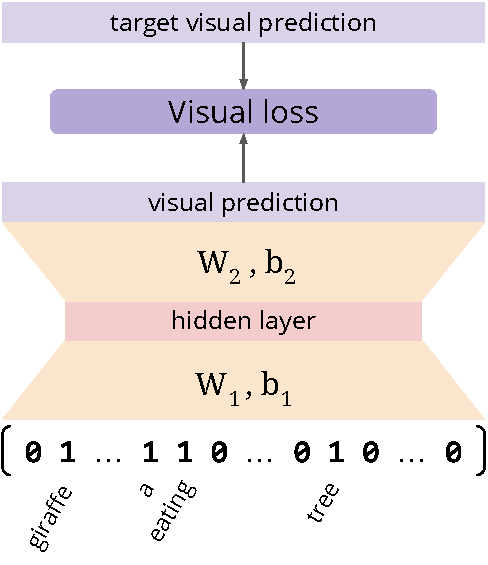
\includegraphics[width=\linewidth]{visreg-arch}
\caption{Architecture of a simple regressor model with one hidden layer of size $1,024$.}
\label{fig:t2v:visreg:arch}
\end{subfigure}
\hfill
\begin{subfigure}{0.55\textwidth}
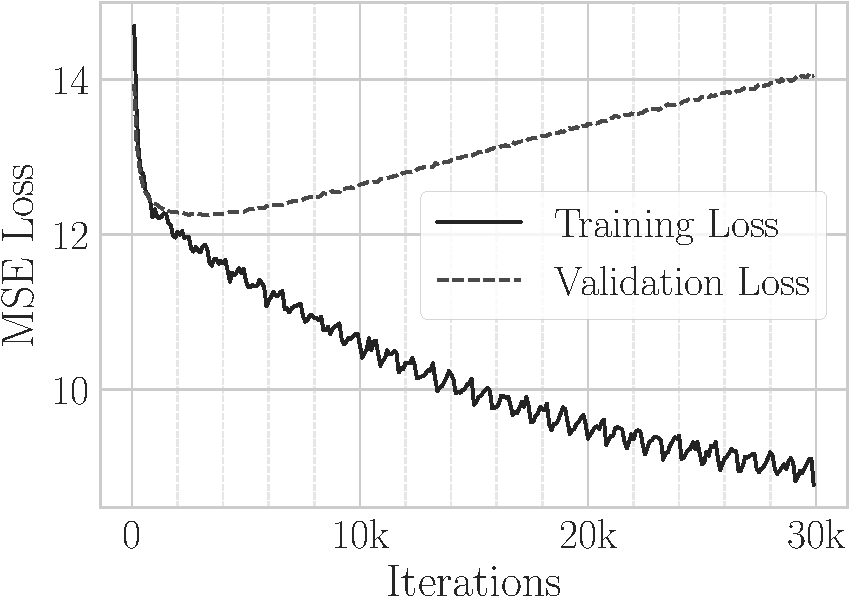
\includegraphics[width=\linewidth]{visreg-loss}
\caption{The training and validation loss (on y-axis) in function of the training iteration (on x-axis).
Notice the model overfits in the early phase of the training process.}
\label{fig:t2v:visreg:loss}
\end{subfigure}
\caption{Baseline \visreg{} model. }
\label{fig:t2v:visreg}
\end{figure}

We explain this overfitting with the fact that a visual representation keeps track of every element that appears in the image, regardless of their semantic relevance within the image, while a (short) textual description is more likely focused on the visually relevant information, disregarding the secondary content of the image.
For example, the relevant images for the query ``a person doing jogging'' will likely share a subset of common features that denote the presence of a person with a posture that is associated to the action of gentle running, and then have many other features related the different compositions of colors, perspective, background elements each image may contain.
As the learning iterations proceed, the simple regressor model starts capturing these secondary elements of the images that are not relevant for the main represented concept, but are somewhat characteristic to the specific set of images that compose the training data.

This preliminary experiment suggests that text-to-image mapping must be somehow regularized.
In the following, we propose various strategies aiming at constraining the mapping to better model the textual part.
%------------------------------------------
\subsection{\sparsettv{}}
\label{subsec:t2v:sparse-t2v}

%As described in the following, \sparsettv{} actually learns a description embedding space that is able to reconstruct both the original description and the visual description.

The first model we propose, dubbed \sparsettv{}, is based on forcing the hidden representation to be representative not only for the visual reconstruction, but also for reconstructing the sparse textual signal.

\sparsettv{} thus contrasts the overfitting by adding a text-to-text autoencoding branch to the hidden layer (\ref{fig:t2v:s-t2v:arch}), constraining the model to jointly satisfy two different losses: one visual (text-to-visual regression) and one linguistic (text-to-text autoencoder).
The linguistic loss works at higher level of abstraction than the visual one, acting as an additional constraint on the model, and preventing (as confirmed by our experiments) overfitting on the visual loss (\ref{fig:t2v:s-t2v:loss}).

%As detailed in the next section, we implemented the use of the two losses with a stochastic process, in which at each iteration one of the two is selected for optimization.

\begin{figure}
\begin{subfigure}{0.53\linewidth}
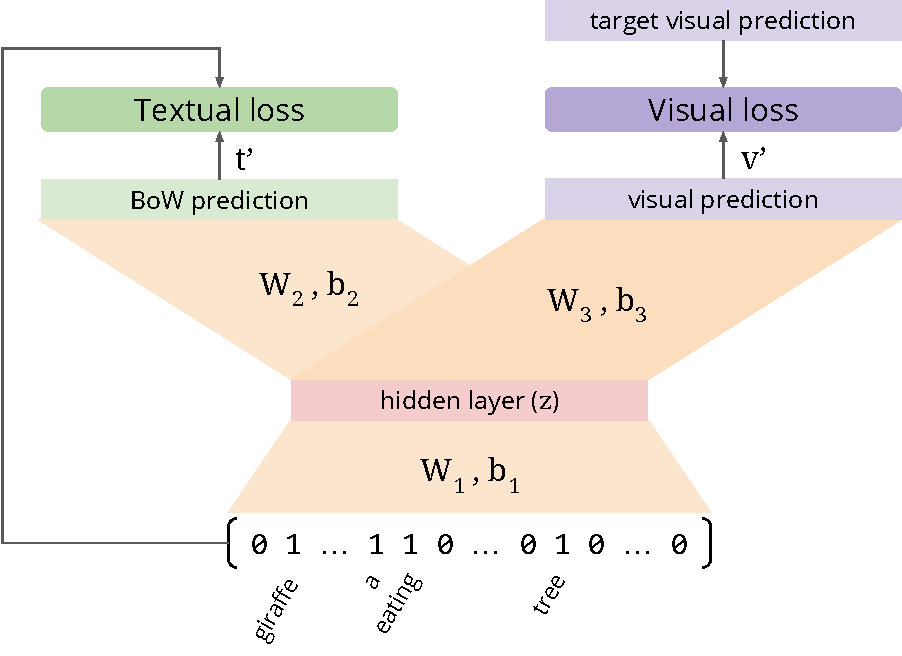
\includegraphics[width=\linewidth]{s-t2v-arch}
\caption{Architecture of our proposed \sparsettv{} which controls overfitting by adding an autoencoding constraint on the hidden state.}
\label{fig:t2v:s-t2v:arch}
\end{subfigure}
\hfill
\begin{subfigure}{0.43\linewidth}
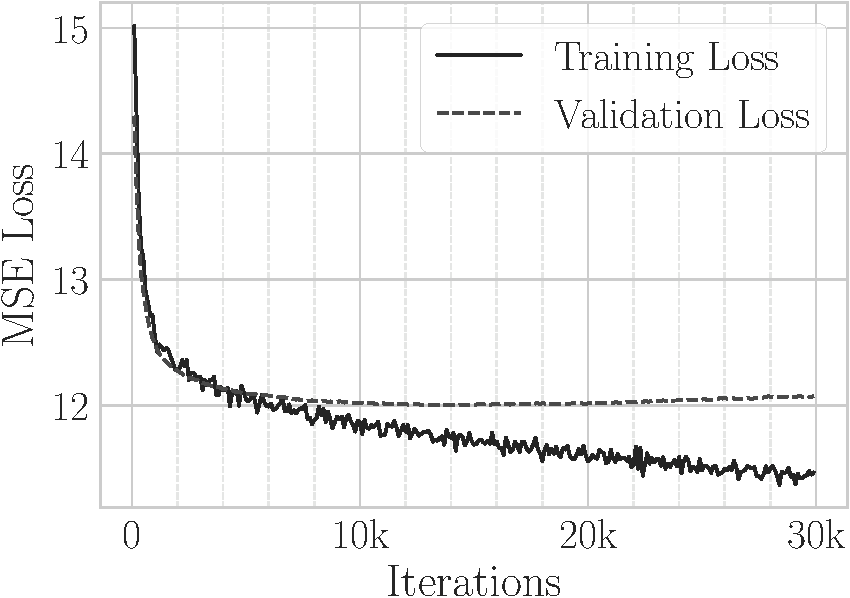
\includegraphics[width=\linewidth]{s-t2v-loss}
\caption{The training and validation loss (on y-axis) in function of the training iteration (on x-axis).}
\label{fig:t2v:s-t2v:loss}
\end{subfigure}
\caption{Our proposed \sparsettv{} model.}
\label{fig:t2v:s-t2v}
\end{figure}

\sparsettv{} consists of two overlapped feed-forward neural nets with a shared hidden layer.
%The shared hidden layer causes a regularization effect during the combined optimization; i.e., the hidden state is constrained to be a good representation to accomplish with two different goals.
The feed-forward computation is described by the following equations:
%
\begin{align} \label{eq:t2v:s-t2v}
%\begin{split}
\z  & = \text{ReLU} \( \W_1 \t + \b_1 \) \\
\t' & = \text{ReLU} \( \W_2 \z + \b_2 \) \\
\v' & = \text{ReLU} \( \W_3 \z + \b_3 \) \,,
%\end{split}
\end{align}
%
\noindent where $\t$ represents the sparse one-hot encoding for the textual descriptor given as input to the net, $\z$ is the hidden representation, $\v'$ and $\t'$ are the visual and textual predictions, respectively, obtained from the hidden representation $\z$, $\Theta=\{W_i,b_i\}, i \in \{1,2,3\}$ are the model parameters to be learned. %, and $ReLU$ is the activation function, defined by $ReLU(x)=\max\{0,x\}$.

Both predictions $\v'$ and $\t'$ are then compared with the expected outputs, i.e.,  the visual embedding representation $\v$, and a textual descriptor $\t'$ that is either $\t$ or semantically equivalent to $\t$ (we expand on this below).
We used the \acrfull{mse} as the loss function both for the visual loss and the textual loss, denoted by $\L_v$ and $\L_t$, respectively.
%
%\begin{equation}
%MSE(y,y') = \frac{1}{n}\sum_{i=1}^{n}(y_i-y'_i)^2 \label{eq:mse}
%\end{equation}
%
%where $y,y'$ are a pair of target description and prediction either in the textual ($t,t'$, left part of the network in \ref{fig:t2v:net-scheme})  or in the visual ($v,v'$, right part of the network in \ref{fig:t2v:net-scheme}) space.}
The model is thus multi-objective, and many alternative strategies could be followed at this point in order to set the $\Theta$ parameters so that both criteria are jointly minimized.
A simple strategy to jointly optimize the two losses consists of defining a single loss as a parametrized aggregation
\begin{equation} \label{eq:t2v:optim}
\Theta^\star =  \argmin_\Theta \( \L_t(\t, \t') + \alpha \L_v(\v, \v') + \lambda ||\Theta||_2 \) \,,
\end{equation}
where $\alhpa$ is a parameter controlling the relative contribution of the losses~\cite{feng2014cross}.
We also add an $L_2$ regularization term parametrized by $\lambda$ to further counter overfitting.
Note that the net is fed with a triplet $\left \langle \v, \t, \t' \right \rangle$ at each iteration.
When $\t'=\t$ the text-to-text branch is an \emph{autoencoder}.
It is also possible to have $\t \neq \t'$, with the two pieces of text being semantically equivalent --- e.g., $\t = $``\texttt{a woman cutting a pizza with a knife}'', $\t'=$``\texttt{a woman holds a knife to cut pizza}'').
%In the latter case the text-to-text branch might be reminiscent of the \emph{SkipGram} and \emph{CBOW} architectures.
The text-to-image branch is, in any case, a regressor.
Notwithstanding, since our final goal is to project the textual descriptor into the visual space, the text-to-text branch might be though as an additional constraint (of linguistic nature)
%regularization
to the visual reconstruction (and, more specifically, to its internal encoding).% which responds to constrains of linguistic nature.

The main strength of \sparsettv{} regards its simplicity, specially in the use of the most simple representation for the input (the sparse encoding); yet it produces effective results (as discussed bellow).
That being said, the model presents some flaws too, i.e.,
(i) the sparse encoding results in a high dimensionality, thus constraining the net to optimize a large number of parameters, and
(ii) the model is agnostic to word order, thus losing relevant information from text, e.g.: ``\texttt{a white cat and a black dog}'' vs ``\texttt{a black cat and a white dog}''.

%----------------------------------------
\subsection{\densettv{}}
\label{subsec:t2v:dense-t2v}

The second model we propose, dubbed \densettv{}, is meant to overcome the limitations of \sparsettv{}.

In order to reduce the amount of parameters of the net, we resort to dense representations (i.e.,  word embeddings) for the terms in the description.
Besides the mere reduction in the number of dimensions, the main reason that motivates operating in a dense embedding space concerns with the gain in generalization.
Words with similar meanings end up being represented by similar vectors (in the sense of the inner product), which allows the model to better generalize, i.e.,  the patterns discovered become descriptive for an embedding region (and to the greater or lesser extent to words with nearby embeddings) rather than descriptive for a single word.

In order to make the model become sensible to word order, we adopt an \acrfull{lstm}~\cite{hochreiter1997long} architecture, a special kind of recurrent neural network which is particularly robust to learn from sequential data (such as textual data).
Concretely, we train an \gls{lstm} on the task of language modeling (that is, the task of predicting the most likely following term given the sequence of preceding terms -- see e.g., ~\cite{sundermeyer2012lstm}) with backpropagation through time~\cite{werbos1990backpropagation}.
We constrain the internal memory state of the last memory cell to be a good representation to predict the visual embedding (\ref{fig:t2v:d-t2v-arch}).

\begin{figure}
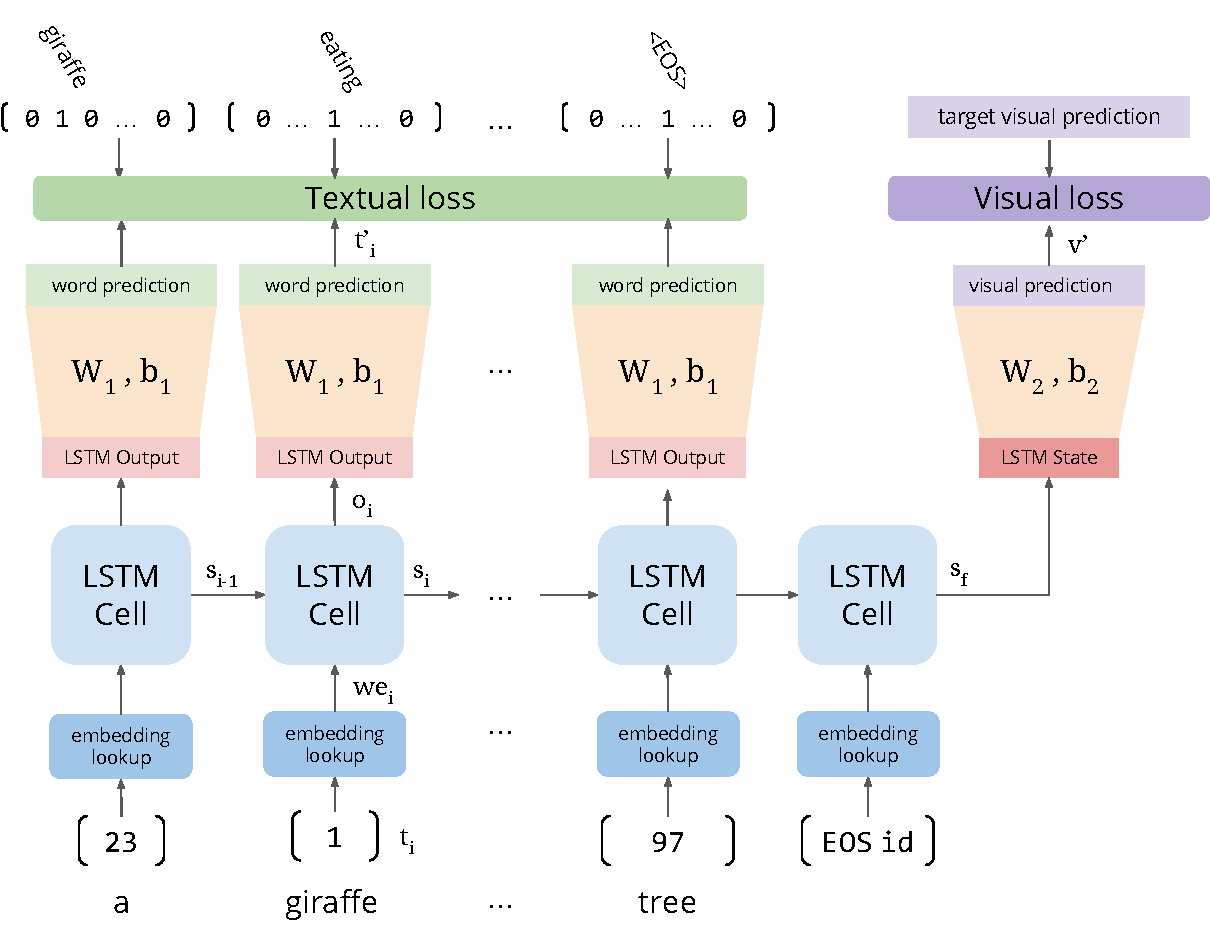
\includegraphics[width=\linewidth]{d-t2v-arch}
\caption{Architecture of \densettv{}.}
\label{fig:t2v:d-t2v-arch}
\end{figure}

The computation is described by the following equations:
%
\begin{align} \label{eq:t2v:d-t2v}
%\begin{split}
\e_i  & = \text{lookup} \( \E, \t_i \) \\ \label{eq:t2v:d-t2v:1}
\o_i, \s_i & = \text{LSTM} \( \e_i, \s_{i-1} \) \\ \label{eq:t2v:d-t2v:2}
\t'_i  & = \text{softmax} \( \W_1 \o_i + \b_1 \) \\ \label{eq:t2v:d-t2v:3}
\v' & =  \text{ReLU} \( \W_2 \s_f + \b_2 \) \,,
%\end{split}
\end{align}
%
where $\text{lookup}()$ returns the word-embedding $\e_i$ from the (trainable) matrix $\E$ for the $i$-th word in the textual descriptor with index $\t_i$, $\text{LSTM}$ is the memory cell, $\o_i$ and $\s_i$ represent the \emph{output} and \emph{hidden state} signals produced after processing $\e_i$ and $\s_{i-1}$ (the state signal produced in the precedent step), and $\s_f$ is the state of the last memory cell.
The softmax function transforms the output signal into a probability distribution on the vocabulary-length space. Finally, $\v'$ and $\t'_i$ are the visual vector and term predictions, respectively.

Note that in addition to the parameters $\E$, $\W_{\{1,2\}}$ and $\b_{\{1,2\}}$, the \gls{lstm} cell internally maintains an \emph{input}, \emph{output}, and \emph{forget} gates with their own parameters; as the memory cell we used the implementation described in~\cite{sak2014long}.

The sequence of term vectors predictions $\t'_i$ and the visual prediction $\v'$ are then compared to the expected textual and visual outputs.
%, i.e., the sequence of words $w_i$ and the visual embedding $v$, respectively.
For the visual loss $\L_v$ we use the \gls{mse} as before.
Each predicted term $\t'_i$ is a $|V|$-dimensional vector that could be though as a probability distribution over the term indexes, where $V$ is the vocabulary.

Analogously, each term $w$ can be codified as a \emph{one-hot} vector, i.e.,  a $|V|$-dimensional vector with all zero values except the dedicated dimension indexing $\t_i$, which is set to one.
Note that a one-hot encoding could be interpreted as a probability distribution as well.
(When not confusing, we use $\t_i$ both to refer to the term symbol and to its one-hot encoding.)
The error between both distributions is compared via the cross-entropy loss $\L_{CE}$.
Given the sequence $\t$ of expected terms $\t_i$ and the sequence $\t'$ of predicted signals $\t'_i$ outputted by the net, the textual loss is computed as the averaged cross-entropy
%For the sequence of predicted textual outputs we use the (averaged) cross-entropy error (Equation \ref{eq:crossentropy}) as the loss function $\L_t$.
%
\begin{equation} \label{eq:t2v:textual-loss}
\L_t \( \t,\t' \) = \frac{1}{n} \sum_{i=1}^{n} \L_{CE} \( \t_i, \t'_i \) \,,
\end{equation}
%
%The model is, again, multi-objective.
%In this case, we found that a simple sum of the losses, without a weighting parameter, allowed the optimizer algorithm to find a good set of parameters (as demonstrated by our experiments).
%For this reason we did not explore the use of SL, left to future investigation.
%where $y,y'$ represent any pair of true and predicted distributions.
As before, the net is fed with a triple $\left \langle \v, \t, \t' \right \rangle$ where, given a caption $[\t_0 \ldots \t_{L}]$, the input ant output textual sequences are defined as $ \t = [\t_0 \ldots \t_{L-1}]$ and $ \t' = [\t_1 \ldots \t_{L}]$, being $\t_L=\text{EOS}$ a special symbol delimiting end of the sequence.
That is, the expected sequence corresponds to the input sequence shifted one position since the \gls{lstm} part is trained to predict the next term in the sequence.
As the model is, again, multi-objective, we apply the weighted aggregation described by \ref{eq:t2v:optim} to set the optimization problem.

%Given an input sequence $t_{in}=[w_0\ldots w_{L-1}]$, where $w_0=$START is a special symbol indicating the beginning of the sentence; the expected output sentence $t_{out}=[w_1\ldots w_{L}]$, where $w_L=$END denotes the end of the sentence; and the sequence of term predictions $[t'_1\ldots t'_{L}]$ outputted by the net, the textual loss is computed as the averaged cross-entropy (\ref{eq:t2v:textual-loss}).
%<here>
%Let us define $t_{in}=[w_0\ldots w_{L-1}]$ as the input textual sequence, $t_{out}=[w_1\ldots w_{L}]$ as the output textual sequence, and $v$ as the true visual embeddings.
%Let us also define the trivial function $onehot(w_i)$ which returns a vector with all elements equal to zero except the index of the i\textit{th} element, which is equal to one.
%Having fixed the notation, the optimization problem is set as follows:
%
%\begin{eqnarray}
%\{v',[t'_1\ldots t'_{L}]\} := \densettv{}(t_{in};\Theta) \\
%\hat{\Theta}  =  argmin_{\Theta} \left( \L_v(v,v') + \alpha\L_t(t_{out},t') + \lambda||\Theta||_2 \right)
%\end{eqnarray}
%

%----------------------------------------
\subsection{\widedeepttv{}}
\label{subsec:t2v:wd-ttv}

Our last proposal, dubbed \widedeepttv{}, combines the sparse and dense representations by following the recently proposed \emph{Wide \& Deep Learning} strategy~\cite{cheng2016wide}.

\widedeepttv{} combines the deep \gls{lstm} (borrowed from \densettv{}) with a wide regressor.
Linear models with non-linear feature transformations are known to be useful for large-scale regression problems with sparse inputs (as is the case for short text descriptions).
This model emerged from the belief, discussed in \cite{cheng2016wide}, that the deep part contributes to model \emph{generalization} while the wide part contributes to model \emph{memory}, and therefore their combination might be beneficial.

\begin{figure}
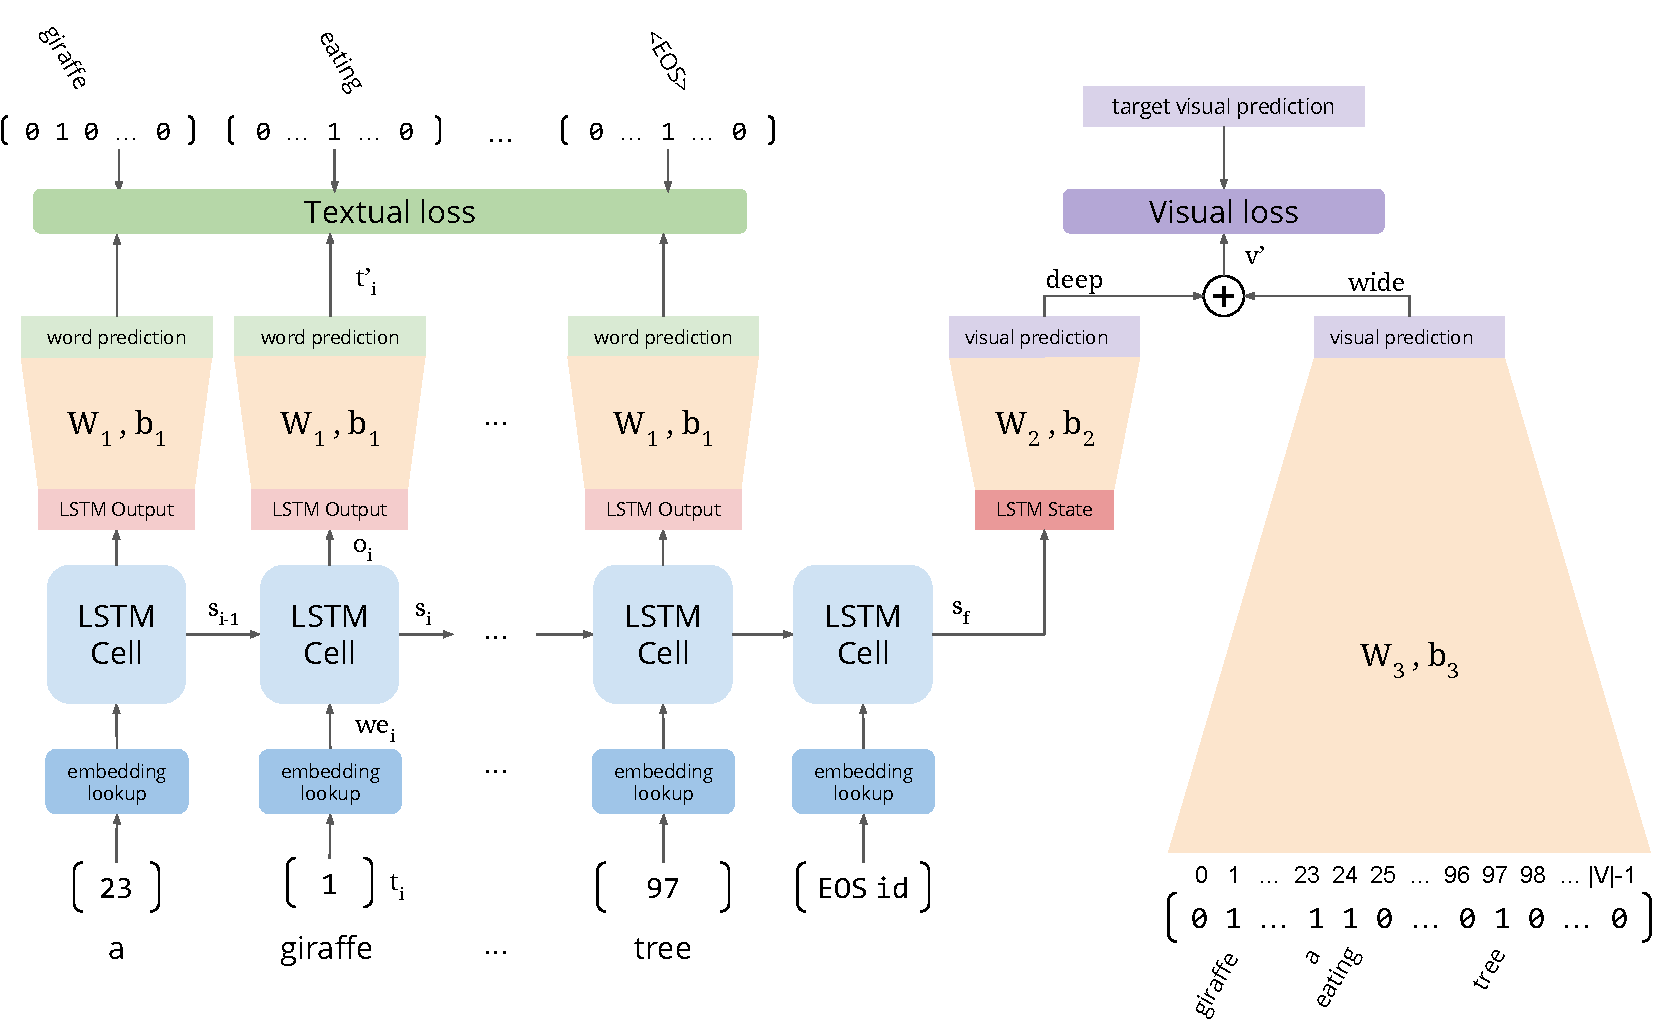
\includegraphics[width=\linewidth]{wd-t2v-arch}
\caption{Architecture of \widedeepttv{}.}
\label{fig:t2v:widendeep}
\end{figure}

The fundamental difference with respect to \cite{cheng2016wide} is that we use a recurrent neural network as the deep part (instead of a feed-forward network) since \glspl{lstm} are particularly fit to learn from sequential data such as our textual descriptions.

The computations reuse \ref{eq:t2v:d-t2v:1,eq:t2v:d-t2v:2,eq:t2v:d-t2v:3} from \densettv{} and incorporate the following set of equations for the wide part:
\begin{align} \label{eq:t2v:wd-t2v}
%we_i &=& lookup(WE,w_i)\\
%o_i,s_i &=& LSTMcell(we_i,s_{i-1})\\
%t'_{i} &=& \sigma(W_{1} o_i + b_{1})\\
\text{deep} &= \W_2 \s_f + \b_2 \\
\text{wide} &= \W_3 \( \sum_{i=0}^L \text{onehot}(\t_i) \) + \b_3 \\
\v'  &= \text{ReLU} \( \text{wide} + \text{deep} \) \,,
\end{align}
where $\text{onehot}(\t_i)$ returns the one-hot encoding vector for term $\t_i$.
As in \densettv{}, we used the \gls{mse} loss for the visual loss $\L_v$ and the averaged cross-entropy (\ref{eq:t2v:textual-loss}) for the textual loss $\L_t$.
The optimization problem is set as in \ref{eq:t2v:optim}.
%The definitions of the loss functions and the optimization is as in \densettv{}, i.e., the visual loss $\L_v$ is the $MSE$ (\ref{eq:mse}) and the textual loss $\L_t$ is the cross entropy (\ref{eq:crossentropy}). The optimization search is thus defined as:
%
%\begin{eqnarray}
%\{v',[t'_1\ldots t'_{L}]\} := \widedeepttv{}(t_{in};\Theta) \\
% \hat{\Theta}  =  argmin_{\Theta} \left( \L_v(v,v') + \frac{1}{L}\sum_{i\in\{1..L\}}\L_t(onehot(w_i),t'_i) \right)
%\end{eqnarray}
%

%------------------------------------------------------------
\section{Experiments}
\label{sec:t2v:experiments}

In this section, we describe the set of experiments we have carried out in order to test our methods.

\subsection{Datasets}

We used the \emph{Microsoft \acrfull{coco}} dataset\footnote{Publicly available at \url{http://mscoco.org/}}~\cite{lin2014microsoft}).
\gls{coco} was originally proposed for image recognition, segmentation, and caption generation.
Although other datasets for image retrieval exist (e.g., the one proposed by \citet{hua2013clickage}), they are more oriented to keyword-based queries.
We believe \gls{coco} to be more fit to the scenario we want to explore, since the captions associated to the images are expressed in natural language, thus semantically richer than a short list of keywords composing a query.

\gls{coco} contains $82,783$ training images (\emph{Train2014}), $40,504$ validation images (\emph{Val2014}), and about 40K and 80K test images corresponding to two different competitions~\cite{chen2015microsoft} (\emph{Test2014} and \emph{Test2015}).
Since \gls{coco} was proposed for caption generation, the captions are only accessible in the \emph{Train2014} and \emph{Val2014} sets, while they are not yet released for \emph{Test2014} and \emph{Test2015}. % TODO check this statement
We have thus taken the \emph{Train2014} set for training, and randomly split the \emph{Val2014} into two disjoint sets of 20K images each for validation and test.

Each image in \gls{coco} has five different captions associated\footnote{Actually in the dataset there are few images with more than five captions available for processing. In such cases we took the first five listed.}, each of which written by a different individual.
Let $\langle I, C \rangle$ be any labeled instance in \gls{coco}, where $I$ is an image and $C = \{ c_1, \ldots, c_5\}$ is a set of captions describing the content of $I$.
Given a $\langle I, C \rangle$ pair, we define a training labeled instance in our model as $\left \langle \v,\t \right \rangle$ where $\v \in \R^{2,048}$ is the visual representation of the image $I$ taken from the \emph{pool5} layer, or $\v \in \R^{4,096}$ when the representation comes from the \emph{fc6} or \emph{fc7} layer (each representation has been tested in distinct experiments), and $\t$ is a textual descriptor randomly chosen from $C$ representing the input descriptor for the model.
In the exceptional case of \sparsettv{} a training label instance is defined as $\left \langle \v, \t, \t' \right\rangle$, where $\t'$ is the output textual descriptor randomly chosen from $C$ (the meanings for $\v$ and $\t$ remain untouched).
Note that, in this case, $\t$ and $\t'$ are not imposed to be different, thus leading to a total of 25 possible combinations of training instances one could extract from a single pair $\langle I, C \rangle$;
this increases the variability of the training set a lot along the different epochs.
The training triplet $\langle \v, \t, \t' \rangle$ for \densettv{} and \widedeepttv{} models are extracted from the instance $\langle I, C \rangle$ by randomly choosing $\t$ from $C$ and then defining $\t'$ as $\t$ shifted one position (as explained above, see \ref{subsec:t2v:dense-t2v}).

%--------------------------------------------------------

\subsection{Visual similarity search}

We evaluated the visual similarity between any two images by comparing their visual descriptions obtained as described in \ref{sec:t2v:method}.
In particular, given the improvement in performance in \gls{cbir} task reported in \cite{sharif2014cnn,gong2014multi,gordo2016deep}, the Euclidean distance is used to compare the vectors obtained applying \gls{pca} and whitening \cite{comon1994independent} to the neurons activation.
The resulting vectors have components which are uncorrelated and have unit variance.
In our experiments, we considered the first 256 components obtained after \gls{pca} (while the original dimension was $2,048$ in the \emph{pool5} layer, and $4,096$ in \emph{fc6} and \emph{fc7} layers).

%--------------------------------------------------------

\subsection{Training}

We tackle the optimization problems using the Adam optimizer~\cite{kingma2014adam} with default parameters (learning rate $0.001$, $\beta_1=0.9$, $\beta_2=0.999$, and $\epsilon=1e^{-0.8}$) in all cases.

We set the size of the training batch to 64 examples, each of which was extracted from a different image.
Each training example in the batch corresponds to the visual features $\v$ of a different image $I$, and a textual descriptor $\t$ picked at random from the set $C$ of captions associated to $I$ in \gls{coco}.
As explained above, \sparsettv{} requires an additional $\t'$ which is also picked at random from $C$ during training.
During test, we consider all captions as different queries.
We set the maximum number of iterations to $300,000$ in \sparsettv{}, and to $50,000$ in \densettv{} and \widedeepttv{}, but apply an early-stop policy when the model starts overfitting (as reflected in the validation error).
The training set is shuffled each time a complete pass over all images is performed.

The word embedding matrix for \densettv{} and \widedeepttv{} has been initialized at random according to an uniform distribution ranging from $-1.0$ to $1.0$.
In preliminary experiments, we investigated on the use of pre-trained word embeddings, i.e.,  representing the textual description as the average of the embeddings of the words composing the description (see~\cite{dong2018predicting}), but we have not observed any improvement.
Pre-training the word embeddings is an additional cost, and the fitness of the embeddings for the task depends on the type of documents they are learned from.
For example, an 11\% improvement in \gls{map} is reported in \cite{cappallo2015image2emoji} from learning embeddings from Flickr tags compared to learning them from Wikipedia pages.

The rest of the $\Theta$ parameters for all models (with the sole exception of the word embedding matrix) have been initialized at random according to a truncated normal distribution centered in zero with standard deviation of $\frac{1}{\sqrt{n}}$, where $n$ is the number of columns.
The biases have all been initialized to 0.

%\subsection{Why Stochastic Loss?}\label{sec:t2v:sl}
%In order to train the \sparsettv{} model we resort to two independent optimizers to optimize the visual ($\L_v$) and the textual ($\L_t$) losses (SL, Equations \ref{eq:op:t} and \ref{eq:op:v}).
%Previous approaches to multimodal learning relied instead on a unique aggregated loss (typically of the form $\L=\L_v+\lambda\L_t$) that is minimized by a single optimizer \cite{feng2014cross,ngiam2011multimodal}.
%However, in this particular case we found the SL to be convenient.
%We compared the two approaches on the case of equal relevance of the two losses ($\lambda=1$, uniform distribution for SL).
%SL better optimizes the two losses (\ref{fig:t2v:modaltrends}), and is less prone to overfit.
%We deem that SL allows to model in a more natural way the relative relevance of the various losses that are combined, i.e., by selecting the losses in proportion to the assigned relevance, whereas the numeric aggregation is affected by the relative values of losses and the differences in their variation during the optimization (e.g., a loss that has a large improvement may compensate for another loss getting worse).
%SL is also computationally lighter than the aggregated loss, as SL updates only a part of the model on each iteration.
Following previous approaches to multimodal learning \cite{feng2014cross,ngiam2011multimodal}, we adopted an aggregated loss which depends on one single parameter $\alpha$ (\ref{eq:t2v:optim}).
In~\cite{feng2014cross}, it was found that unbalancing aggressively the loss pressure towards one or the other extremes tends to degrade the performance.
For the $\alpha$ hyperparameter, we have tried the values $\{0.01, 0.1, 1.0, 10.0, 100.0\}$, choosing the best one for each visual embedding layer as reflected in the validation error.
For the parameter $\lambda$ determining the impact of the $L_2$ regularization, we tried the values $10^i, i\in\{1,-2,-4,-6\}$.

% %
% \begin{figure}[ht!]
% \center
% \includegraphics[width=0.45\textwidth]{S-Text2Vis-visualloss}
% \qquad
% \includegraphics[width=0.45\textwidth]{S-Text2Vis-captionloss}
% \caption{Validation loss for $\L_v$ and $\L_t$, optimizing on a linear combination of losses (blue) or using two  optimizers with stochastic loss selection (SL, red).}
% \label{fig:t2v:modaltrends}
% \end{figure}

For \sparsettv{}, we tested two different vectorial representations of text: \sparsettv{}\textsc{-U} uses a simple \acrlong{bow} vectors that marks with a value of one the positions that are relative to words that appear in the textual description and leave to zero all the others; \sparsettv{}\textsc{-N} adds a little bit of information on the text structure by considering also N-grams for a selection of part-of-speech patterns\footnote{We considered the part-of-speech patterns: `NOUN-VERB', `NOUN-VERB-VERB', `ADJ-NOUN', `VERB-PRT', `VERB-VERB', `NUM-NOUN', and `NOUN-NOUN'.}.
%\sparsettv{}$-N$ is a first approach at modeling text structure into the input vectorial representation, which differentiates the task of search from detailed/complex textual description we aim at from the traditional keyword search.
The resulting vocabulary size $|V|$ is $10,358$ for \sparsettv{}\textsc{-U} after removing terms appearing in less than 5 captions.
For \sparsettv{}\textsc{-N} we considered the $23,968$ uni-grams and N-grams appearing at least in 10 captions.
We set the number of nodes of the hidden layer to $1,024$ which was experimentally confirmed as the best value among the candidates $\{ 256, 512, 1024, 2048 \}$;
we omit those experiments for the sake of conciseness.

In order to efficiently train the \gls{lstm} part in \densettv{} and \widedeepttv{}, we make use of \emph{padding} and \emph{bucketing}.
That is, to avoid constructing as many computational graphs as different caption lengths there are in the dataset, we fix a number of buckets (i.e.,  sequences of fixed length -- we considered $\{15, 20, 40\}$ in our experiments) and apply padding to the captions (i.e.,  repeatedly adding the `PAD' token at the beginning of the tokens sequence, and the special `EOS' token announcing the end of the sequence) to fit in the corresponding bucket (the smallest one that could allocate the caption).

For \densettv{} and \widedeepttv{}, we have also considered stacking \gls{lstm} cells as a mean to give the model a greater expressive power.
We denote those variations by the suffix `-$\langle n\rangle$' where $n$ indicates the height of the stack.
For example, \densettv{}$-1$ corresponds to the vanilla model in \ref{fig:t2v:d-t2v-arch}, while \widedeepttv{}$-4$ is the wide \& deep approach with 4 \gls{lstm} cells stacked.
In all cases, we set the dimensionality of the embedding space to 100 and the size of the internal \gls{lstm} nodes to 512;
again, those values were chosen during preliminary experiments run on the validation set.

% \begin{table}[ht!]
% \centering
%   \resizebox{\textwidth}{!} {
% \begin{tabular}{|c|c|c|c|c|c|c|c|c|c|}
% \hline
% Model & VisReg & S-U & S-N & D-1 & D-2 & D-4 & W\&D-1 & W\&D-2 & W\&D-4 \\ \hline
% Params  & 14.8M   & 25.4M         & 53.3M        & 10.5M         & 15.7M         & 26M           & 51.5M            & 56.7M             & 67M               \\ \hline
% \end{tabular}
% }
% \caption{Number of parameters to learn per model. Prefix `S-' denotes \sparsettv{}, `D-' denotes \densettv{}, and `W\&D-' denotes \widedeepttv{}}
% \label{tab:t2v:paramsmodel}
% \end{table}

A Tensorflow implementation of all our methods, and of all the compared methods described in the next section, is available at \url{https://github.com/AlexMoreo/tensorflow-Tex2Vis}.

%--------------------------------------------------------
\subsection{Compared methods}
\label{subsec:t2v:compared-methods}

We compare the performance of the various \ttv{} models against a selection of methods that perform search either in the visual space or in the textual space.
We define as the trivial lower bound baseline the method that produces a random ranking of the images in the collection (dubbed \emph{RRank}).

We define as \emph{VisSim} the direct similarity method that computes the Euclidean distances using the original \emph{pool5} (from the \resnet{}~\cite{he2015deep}), and \emph{fc6} or \emph{fc7} features (from the AlexNet~\cite{zhou2014learning}) for the image that is associated to the query caption in \gls{coco}.
\emph{VisSim} models the scenario in which the user submits the query using an image that is representative of the original textual description.
\emph{VisSim} is thus not a real cross-media search model, but it allows us to measure how a search-by-representative-image process compares with the real cross-media search approaches.
We also compare with \visreg{}, the text-to-image sparse regressor described in \ref{subsec:t2v:vis-reg}.

We use the caption generation methods presented in \cite{karpathy2015deep} (dubbed \emph{NeuralTalk}) and \cite{vinyals2015show} (dubbed \emph{Show\&Tell}) to implement cross-media search methods based on textual search.
Given a caption generation method, we generate captions for all the 20K images in the test collection, and then we implement the search process as a text similarity search process based on two retrieval models: one that used the same $\text{ROUGE}_L$ metric that is used for the evaluation (dubbed \emph{CapRouge}), and one that uses a more classic ranking by $L_2$ norm of the vectors resulting from text indexing based on \acrlong{bow} or characters 3- and 4-grams (respectively dubbed \emph{CapBow} and \emph{CapGrams}).
We used two \emph{Show\&Tell} models, one trained for one million iterations (\emph{Show\&Tell-1M}), and another for two million iterations (\emph{Show\&Tell-2M}).
It is important to stress that the \emph{CapRouge} method is to be considered as a very strong but unrealistic baseline, added for the sake of a richer comparison, and not a viable retrieval method, for two reasons.
First, it uses the same metric of the evaluation, so it improperly overfits on it.
Second, it has a computational cost that is quadratic with the length of the compared string, making it not practically usable.
For example, computing the ranking of 20K captions from the test set against a query caption required on average for all the queries, on the same hardware and using efficient implementation, 0.046 seconds for \emph{CapBoW} and \emph{CapGram} methods and 3.267 seconds for \emph{CapRouge}, resulting two orders of magnitude slower than the other methods.
%\todo{Sono in realta' 100,000 captions (20K images x 5 captions), o abbiamo scelto solo la caption 0?}

We also compare our \ttv{} variants against \wordvisual{} \cite{dong2018predicting}, a method that maps the text input into the visual space. % TODO check (as described in \ref{rw:visual}).
We have reimplemented \wordvisual{} by following \cite{dong2018predicting}.
We have pre-trained a 500-dimensional word embeddings space on the user tags associated to 100M images in the YFCC100M dataset \cite{thomee2016yfcc100m} using the skip-gram model in Word2Vec~\cite{mikolov2013distributed}.
We have experimented with two variants: \emph{short} (\wordvisual{}-S), which trains a feed-forward network with two hidden layers of $[1000, 2000]$; and \emph{long} (\wordvisual{}-L), which considers three hidden layers of $[1000, 2000, 3000]$.
We have only experimented with the variant that adopts the same \gls{mse} loss function as our model\footnote{They reported slightly better results with the Marginal Ranking Loss (MRL), a cost function that takes two visual vectors for each example, one considered relevant, and another irrelevant, to the textual description. However, relevance judgments to generate the training triplets relied on the user-click logs available in their dataset.}. %In spite of the user-click logs we preferred not to involve the $ROUGE_L$ measure as a relevance estimator, as it is a fundamental part of the evaluation criterion. We believe the MRL could bring similar improvements to our method, an hypothesis we led to future research.}.
In order to carry out a fair comparison, we have implemented the exact same retrieval for \wordvisual{} as our method (i.e.,  euclidean distance after PCA and whitening -- see \ref{sec:t2v:method}) instead of the originally proposed \emph{cosine similarity}.
The reason for doing so is that we have observed a consistent improvement of about 3\% in our experiments, and verified similar improvements to be achieved in the case of \wordvisual{} as well;
concretely, \wordvisual{} improved its \gls{dcg} average by 0.073 (with a standard deviation of $\pm4.8e^{-3}$) due to the use of this retrieval method in place of the cosine similarity.

%--------------------------------------------------------
\subsection{Evaluation Measures}
\label{subsec:t2v:eval}

We measure the retrieval effectiveness of the various methods we compare by means of the \emph{\acrfull{dcg}}~\cite{jarvelin2002cumulated}.
%
%\begin{equation}
%DCG_p=\sum_{i=1}^{p}\frac{2^{rel_i}-1}{\log_2(i+1)}
%\end{equation}
%
%where $rel_i$ quantifies the \emph{relevance} of the retrieved element at rank position $i$ with respect to the query, and $p$ is the rank at which the metric is computed;
Specifically, we computed $\mathrm{DCG}@25$ in our experiments, as was done in related research~\cite{hua2013clickage,dong2018predicting}.
Given that some of the compared methods (e.g., text-based search) can produce rankings with ties, we actually use the \gls{tdcg}~\cite{mcsherry2008computing}.
Details about the definitions of \gls{dcg} and \gls{tdcg} can be found in \ref{subsec:back:ir-metrics}.

Because the relevance values for \gls{dcg} are not provided in \gls{coco}, we estimate them by using the $\text{ROUGE}_L$~\cite{lin2004rouge} metric, a measure often used for the evaluation of the results of text summarization algorithms and one of the evaluation measures for the \gls{coco} caption generation competition\footnote{\url{https://github.com/tylin/coco-caption}}~\cite{chen2015microsoft}.
This is a metric based on finding the Longest Common Subsequence (LCS) between the two strings being compared\footnote{LCS is a way to find a common exact sequence of words that is similar to matching word n-grams but less stringent (i.e.,  inside the LCS sequence other words may appear).} and then measuring a weighted harmonic mean ($F_\beta$, with $\beta=1.2$) of the coverage ratios of the subsequence with the two strings.
Using a $\beta$ value greater than one ($\beta=1.2$ is the default value in the \gls{coco} evaluation software) gives a little more importance to producing a good coverage of the gold standard caption.
We compute $r_i = \text{ROUGE}_L ( \t, C_i ) $, where $\t$ is the query caption, and $C_i$ are the 5 captions associated to the retrieved image at rank $i$.
This caption-to-caption relevance model is thus aimed at measuring how much the concepts expressed in the query appear as relevant parts of the retrieved images.

As a final note on the evaluation, it is noteworthy that many related methods so far \cite{mao2014deep,ma2015multimodal,klein2014fisher,karpathy2015deep,donahue2015long,kiros2015skip,wang2016learning} have been tested in \gls{coco} as well.
In doing so, however, they have followed a different experimental protocol, involving one random split of 1K test items (not standard across the experiments) and relying on rank-based metrics, namely, \emph{recall at K} (noted by $R@K$ -- the proportion of queries whose expected image was found among the top-$K$ retrieved items) and $medR$ (the median of the rank distribution).
Despite the fact that this protocol has become almost a standard practice in the literature, we argue it might fail to reflect the scenario we are concerned with here, i.e.,  the fact that the ``prototypical'' image one has in mind might be better described through a short textual description of it than through a specific sample image accommodating the textual description (and, unavoidably, much other irrelevant information).
Therefore, the rank of the \emph{specific} test image might not necessarily be a good estimator of the system's ability to generalize well in text-to-image retrieval task.
That is, although it is clear that a well-performing system will deliver competitive rank-based metrics, it is also true that an overfitted system will rank a test image well whenever a very similar example is seen in the training phase.
Contrarily, a text-centered metric (as the \gls{dcg} with $\text{ROUGE}_L$) is not liable to be likewise cheated.
\ref{fig:t2v:metrics} reports some examples, taken from actual results from our methods, in which a good recall does not result in a good selection of top ranked images, and examples in which a zero R@5 is obtained on rankings that contain a good selection of relevant images.

Moreover, rank-based metrics are strongly biased towards the test set size (where only 1K images might fail to represent the web-scale scenario) and very unstable with respect to the particular split one could extract from \gls{coco}.
To show this issue, \ref{tab:t2v:splits1k}, reports the variation of R@1, R@5, R@10, \gls{medR} and \gls{dcg} at the variation of the test set size from 1K to 5K images.
\gls{dcg} is the only measures whose value remain stable, while the other measures have a significant drop.
All other things being equal, we present additional results we have obtained by following this protocol for the sake of comparability (see below);
we also report the \acrfull{mrr}, i.e.,  the average of the inverse ranks) as a possibly more reliable rank-centered metric.

\begin{figure}
 \includegraphics[width=\textwidth]{rank_examples}
 \caption{Evaluation metrics through examples retrieved by our \widedeepttv{}-4 in the fc7 visual space.
The first and second rows of results, despite including the specific query image (ranked 4 and 3, respectively), are mostly unrelated to the textual query;
 yet, they would have obtained a maximum R@5 score.
 The rest of the examples do not include the query image in the top-5 rank, but are relevant to the query (and arguably, better prototypes of the description than the query image itself).
 \gls{dcg} successes to capture this phenomenon.}
 \label{fig:t2v:metrics}
\end{figure}

\begin{table}
\centering
\newcolumntype{R}{>{\raggedleft\arraybackslash}X}
\newcolumntype{d}{D{.}{.}{1}}
\newcolumntype{e}{D{.}{.}{3}}
\begin{tabularx}{\linewidth}{ldddde@{\hfill}dddde}
\toprule
 & \multicolumn{5}{c}{\sc 1K samples} & \multicolumn{5}{c}{\sc 5K samples} \\
 \cmidrule(lr){2-6} \cmidrule(lr){7-11}
 & \multicolumn{1}{R}{\textbf{R@1}} & \multicolumn{1}{R}{\textbf{R@5}} & \multicolumn{1}{R}{\textbf{R@10}} & \multicolumn{1}{R}{\textbf{medR}} & \multicolumn{1}{R}{\textbf{DCG}} & \multicolumn{1}{R}{\textbf{R@1}} & \multicolumn{1}{R}{\textbf{R@5}} & \multicolumn{1}{R}{\textbf{R@10}} & \multicolumn{1}{R}{\textbf{medR}} & \multicolumn{1}{R}{\textbf{DCG}} \\
\midrule
mean & 19.1 & 48.5 & 64.6 & 5.9 & 2.370 & 6.9 & 21.3 & 31.7 & 25.7 & 2.408 \\
% std  & 1.047 & 1.350 & 1.393 & 0.349 & 0.023 & 0.322 & 0.507 & 0.538 & 0.749 & 0.012 \\
std  & 1.0  & 1.4  & 1.4  & 0.3 & 0.023 & 0.3 & 0.5  & 0.5  & 0.7  & 0.012 \\
max  & 21.6 & 52.4 & 67.9 & 7   & 2.426 & 7.6 & 22.5 & 33.3 & 27 & 2.439 \\
min  & 15.5 & 44.8 & 60.1 & 5   & 2.294 & 5.9 & 20.0 & 30.5 & 24 & 2.375 \\\hline
\end{tabularx}
\caption{Variance in evaluation metrics measured on 200 random test splits of 1K images vs. 5K images in \gls{coco}.
Results correspond to the \sparsettv{}-U model projecting into the \emph{pool5} layer.
The rank-centered metrics \gls{r@k} and \gle{medR} present a higher dependency on the sampling size than the \gls{dcg}.
}
\label{tab:t2v:splits1k}
\end{table}


%--------------------------------------------------------
\subsection{Results}
\label{subsec:t2v:results}

\begin{table}
\renewcommand{\tabcolsep}{3pt}
\newcolumntype{R}{>{\raggedleft\arraybackslash}X}
\begin{tabularx}{\linewidth}{lRRRRRRR}
  \toprule
  & \multicolumn{3}{c}{\sc Textual search space}        & \multicolumn{3}{c}{\sc Visual search space}                                       &           \\
    \cmidrule(lr){2-4}                   \cmidrule(lr){5-7}
  Method               & \multicolumn{1}{c}{\bf CapRouge}       & \multicolumn{1}{c}{\bf CapBoW}         & \multicolumn{1}{c}{\bf CapGram}        & \multicolumn{1}{c}{\bf pool5}     & \multicolumn{1}{c}{\bf fc6}            & \multicolumn{1}{c}{\bf fc7}            & \multicolumn{1}{c}{\bf \# params}          \\
  \midrule
  \emph{RRank}         & 1.524          & 1.524          & 1.524          & 1.524         & 1.524          & 1.524          & -         \\
  \midrule
  \emph{NeuralTalk}    & 2.016          & 1.979          & 1.813          & -             & -              & -               & 148.3M    \\
  \emph{Show\&Tell-1M} & 2.290          & 2.032          & 2.062          & -             & -              & -              & 37.6M     \\
  \emph{Show\&Tell-2M} & \textbf{2.360} & \textbf{2.092} & \textbf{2.122} & -             & -              & -              & 37.6M     \\
  \midrule
  \emph{VisSim}        & -              & -              & -              & 2.266         & 2.150          & 2.180          & -         \\
  % penso l'abbiamo fatta con il coseno... seno vanno un po meglio tutti
  \emph{VisReg}        & -              & -              & -              & 2.349         & 2.317          & 2.359          & 14.8M     \\
  \midrule
  \wordvisual{}-S$_{cos}$  & -          & -              & -              & 2.394         & 2.316          & 2.317          & 10.7M     \\
  \wordvisual{}-L$_{cos}$  & -          & -              & -              & 2.405         & 2.317          & 2.318          & 20.8M     \\
  \wordvisual{}-S      & -              & -              & -              & 2.433         & 2.389          & 2.386          & 10.7M     \\
  \wordvisual{}-L      & -              & -              & -              & 2.443         & 2.390          & 2.389          & 20.8M     \\
  \midrule
  \sparsettv{}-U       & -              & -              & -              & 2.428         & 2.381          & 2.387          & 25.4M     \\
  \sparsettv{}-N       & -              & -              & -              & 2.432         & 2.382          & 2.384          & 53.3M     \\
  \midrule
  \densettv{}-1        & -              & -              & -              & 2.418         & 2.372          & 2.381          & 10.5M     \\
  \densettv{}-2        & -              & -              & -              & 2.435         & 2.384          & 2.389          & 15.7M     \\
  \densettv{}-4        & -              & -              & -              & 2.442         & 2.393          & 2.388          & 26.0M     \\
  \midrule
  \widedeepttv{}-1     & -              & -              & -              & 2.435         & 2.382          & 2.385          & 51.5M     \\
  \widedeepttv{}-2     & -              & -              & -              & \textbf{2.447}& 2.392          & \textbf{2.391} & 56.7M     \\
  \widedeepttv{}-4     & -              & -              & -              & 2.446         & \textbf{2.397} & \textbf{2.391} & 67.0M     \\
  \bottomrule
\end{tabularx}
\caption{Performance comparison of the different methods in terms of average \gls{dcg}.
The bold value highlights the best result in each of the search spaces.}
\label{tab:t2v:dcg}
\end{table}

\ref{tab:t2v:dcg} reports the average \gls{dcg} scores obtained by the compared methods after five runs with different seeds. %\blue{Each run classifies every caption as a different query, that is, }
%When using fc6 as the visual space, \sparsettv{}-1 obtains a $8.51\%$ relative improvement with respect to \emph{VisSim} and $1.40\%$ over \visreg{}.
%The improvements of \sparsettv{}-N are respectively of $8.08\%$ and $0.94\%$.
%When using fc7 as the visual space it is \sparsettv{}-N that obtains, yet by a small margin, the best result.
%The relative improvements of \ttv{}$_1$ over emph{VisSim} and \emph{VisReg} are respectively of $8.48\%$ and $0.97\%$, and for \ttv{}$_N$ respectively of $8.60\%$ and $1.09\%$.
These results show a significant improvement of our \ttv{} variants with respect to the compared methods.
The best absolute result is obtained by \widedeepttv{} when using 2 stacked \glspl{lstm} in the visual space \emph{pool5}, which represents the 8\% of relative improvement with respect to the baseline \emph{VisSim}.
In the \emph{fc6} and \emph{fc7} visual spaces, the \widedeepttv{}-4 obtained the best performance, with a relative improvement to \emph{VisSim} of 11.5\% and 9.7\%, respectively.
%In the fc7 visual space, the \widedeepttv{}, also in the stacked configuration with 4 cells, is again the best performing method, with a 8.9\% of relative improvement with respect to \emph{VisSim}.
The \sparsettv{} model also improved, yet by a smaller margin, over the \emph{VisReg} model, showing that an auto-enconding branch in the network is useful to avoid overfitting on visual features.
The best performing method in the textual space is \emph{CapRouge}.
As detailed in \ref{subsec:t2v:compared-methods}, it cannot be considered a realistic retrieval method, given its computational cost and also because it uses the same measure of the evaluation.
We used it to have a strong baseline against which to compare the visual-space based methods, as we discuss in the following.

The \ttv{} methods all compare better by a large margin than the best \emph{CapBoW} and \emph{CapGram} results.
The worst \ttv{} result (\densettv{}-1 in the \emph{fc6} layer) improves by 11.8\% over the best \emph{CapGram} result.
The best \emph{CapRouge} result is in line with the average \ttv{} results, yet it is affected by the computational issue mentioned before.
The best \ttv{} result (\widedeepttv{}-2 on \emph{pool5}) shows a relative improvement of 3.7\% over the best \emph{CapRouge} result, and of 15.3\% of the best \emph{CapGram} result.

When comparing the \ttv{} results among themselves it is not obvious whether the use of sparse features leads to better or worse results than the use of dense features.
For example, the dense-based models (i.e.,  the \densettv{} variants) improve over the sparse-based models (i.e.,  the \sparsettv{} variants) only when resorting to stacking \gls{lstm} cells.
In strict terms of effectiveness (as measured by \gls{dcg}), this blurs any conclusive remark on the preference of either sparse or dense representations.
%For example, in the fc6 visual layer, the dense-based models (i.e., the \densettv{} variants) seem to consistently outperform the sparse-based models (i.e., the \sparsettv{} variants), whereas this behavior is not reproduced in the fc7.
Notwithstanding, this seemingly contradictory result serves to reinforce another interesting insight, i.e.,  the fact that, despite being unclear which representation mechanism is preferable, the wide \& deep architecture effectively takes advantage of the combination, consistently producing better results.

%Another conclusion supported by the experiments is that stacking various LSTM cells helps to improve the modeling capability of the networks.

In the table, we report the results obtained by the implementation of \wordvisual{} that uses the cosine similarity model originally adopted in \cite{dong2018predicting} (dubbed \wordvisual{}-S$_{cos}$ and \wordvisual{}-L$_{cos}$).
Our implementation using \gls{pca} and whitening for the similarity search (dubbed \wordvisual{}-S and \wordvisual{}-L) obtains an average 4.5\% of improvement.

We found the following differences in performance between the best configuration of each variant to be statistically significant (two-tailored t-test): both \densettv{} and \widedeepttv{} are significantly better than \sparsettv{} with a confidence $p<0.005$, while \widedeepttv{} could only be considered better than \wordvisual{} at the smaller confidence of $p<0.05$.
Furthermore, there are no statistically significant differences between \widedeepttv{} and \densettv{}, nor between \densettv{} and \wordvisual{} performances.

In \ref{tab:t2v:coco1k}, we compare our methods against the results reported for other state-of-the-art methods, using their evaluation measures (see \ref{subsec:t2v:eval} for a vaster discussion).
The \ttv{} methods perform worse than the other methods yet by a margin that we deem acceptable (a loss of 1-2 ranks in \gls{medR}) considering that all the other methods use a joint space projection, thus they have the drawbacks on the image collection processing we discussed at the beginning of the chapter. % \ref{sec:t2v:intro}.
The best performing method, m-CNN, is not even really suited for fast retrieval on large collections, since its network models a distance function, not an explicit projection model, and thus every time a query is given all the collection must be processed by the network to compute the distances between the query and each image.

\begin{table}
\newcolumntype{C}{>{\centering\arraybackslash}X}
\centering
\begin{tabularx}{\linewidth}{lCCCCCC}
\toprule
                                      & \multicolumn{6}{c}{\textsc{\gls{coco} 1K test set}} \\
                                        \cmidrule(lr){2-7}
\textbf{Method}                       & \textbf{DCG}  & \textbf{MRR}   & \textbf{R@1}   & \textbf{R@5}   & \textbf{R@10}  & \textbf{medR} \\
\midrule
S-Text2Vis-U                          & 2.341 & 0.339 & 20.1 & 48.9 & 64.2 & 6  \\
D-Text2Vis-4                          & 2.356 & 0.355 & 21.2 & 51.5 & 67.4 & 5  \\
W\&D-Text2Vis-4                       & 2.367 & 0.367 & 22.8 & 52.4 & 67.6 & 5  \\
W\&D-Text2Vis-8                       & 2.370 & 0.372 & 22.8 & 53.2 & 68.5 & 5  \\
\midrule
m-RNN \cite{mao2014deep}              & -     & -     & 29.0  & 42.2  & 77.0  & 3  \\
m-CNN \cite{ma2015multimodal}         & -     & -     & 32.6  & 68.6  & 82.8  & 3  \\
CCA [FV-HGLMM] \cite{klein2014fisher} & -     & -     & 25.6  & 60.4  & 76.8  & 4  \\
DVSA / BRNN \cite{karpathy2015deep}   & -     & -     & 27.4  & 60.2  & 74.8  & 3  \\
LRCN \cite{donahue2015long}           & -     & -     & 29.0  & 61.6  & 74.8  & 3  \\
STV \cite{kiros2015skip}              & -     & -     & 25.9  & 60.0  & 74.6  & 4  \\
%DSPE \cite{wang2016learning}          & -     & -     & 39.6  & 75.2  & 86.9  & -  \\
\bottomrule
\end{tabularx}
\caption{Comparison of results on \gls{coco} 1K test set for a selection of \ttv{} methods projecting into \emph{pool5}.}
\label{tab:t2v:coco1k}
\end{table}

An interesting aspect that deserves attention concerns with the models complexity, as measured by the amount of parameters to train.
We have investigated the trade-off between the model complexity and the results delivered (\ref{fig:t2v:performance-size}).
The plot shows that the \densettv{} variants require a significantly reduced number of parameters while still being competitive in performance, followed by the \sparsettv{} variants, that however produce fluctuating results in terms of \gls{dcg}, and finally followed by the \widedeepttv{} variants, that despite requiring many parameters to train, consistently deliver good results in all visual spaces.

\begin{figure}
\begin{subfigure}{.31\linewidth}
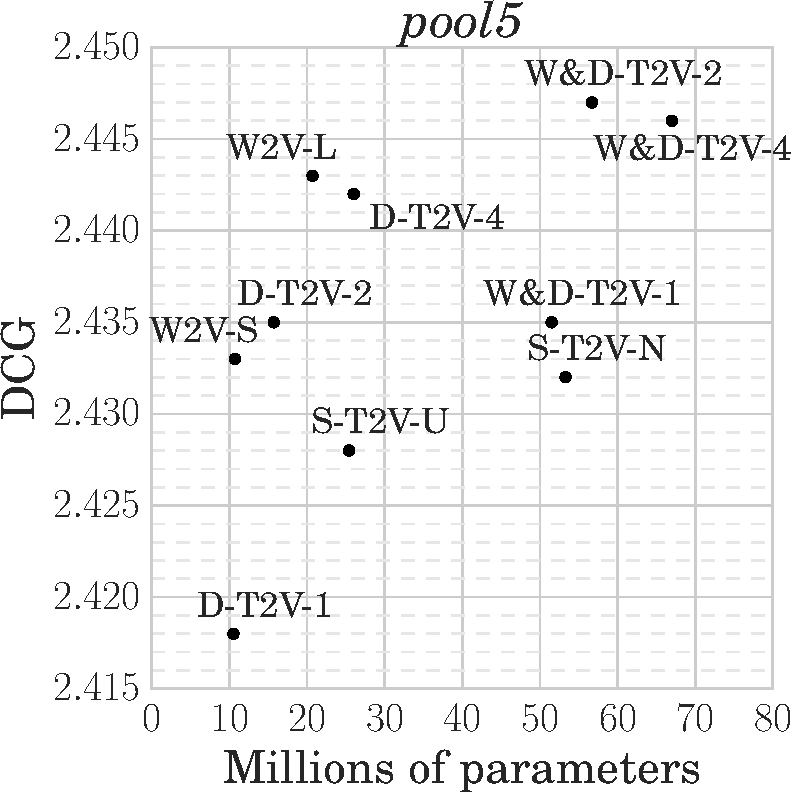
\includegraphics[width=\linewidth]{performance-size-pool5}
\end{subfigure}%
\hfill
\begin{subfigure}{.31\linewidth}
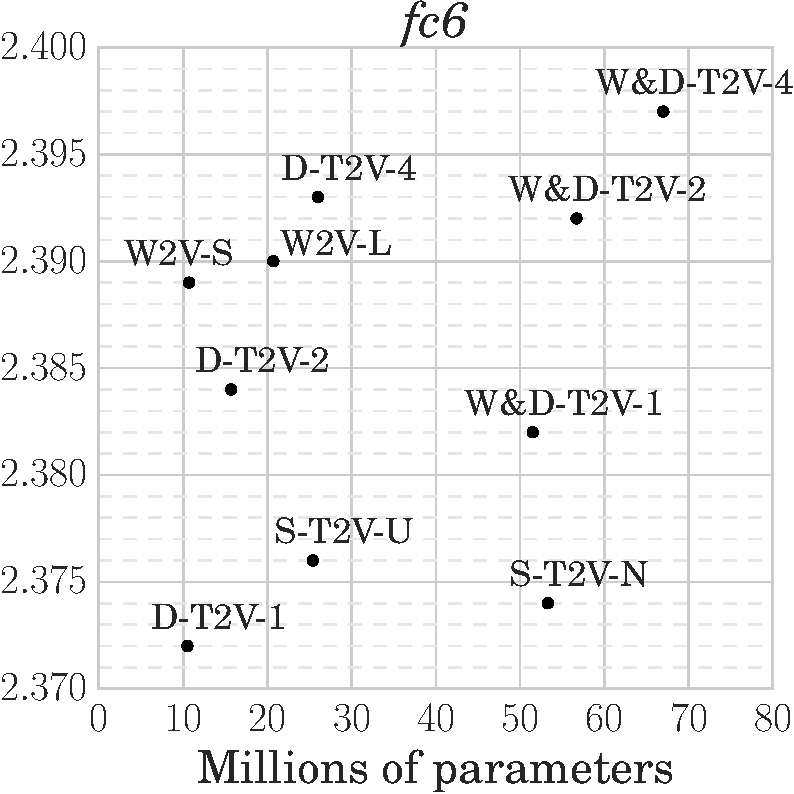
\includegraphics[width=\linewidth]{performance-size-fc6}
\end{subfigure}%
\hfill
\begin{subfigure}{.31\linewidth}
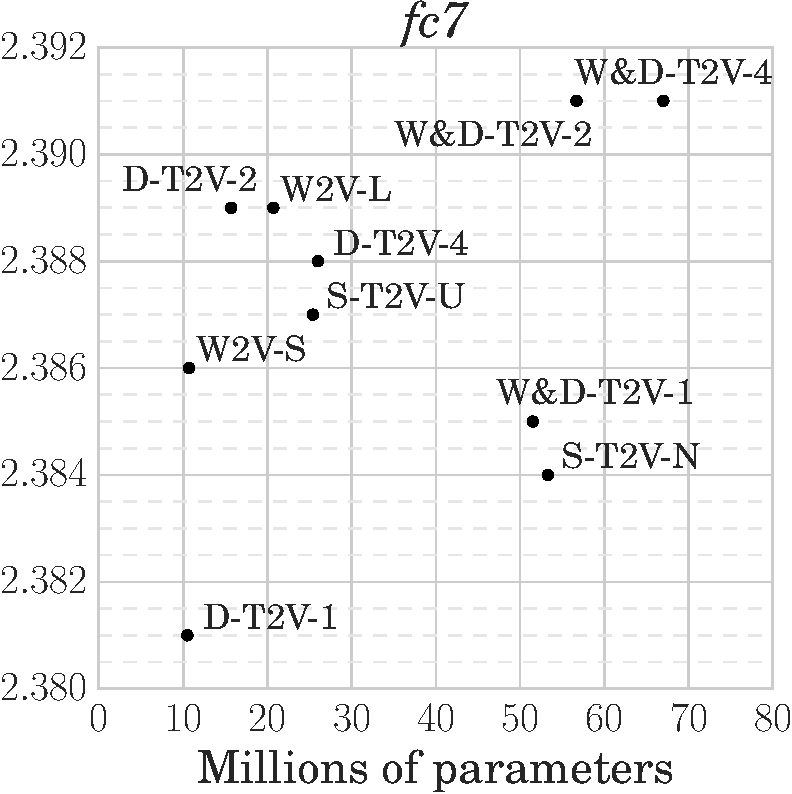
\includegraphics[width=\linewidth]{performance-size-fc7}
\end{subfigure}
\caption{Performance vs number of parameters to learn per model for all feature spaces (\emph{pool5}, \emph{fc6}, and \emph{fc7} from left to right).
Prefix `S-' denotes \sparsettv{}, `D-' denotes \densettv{}, `W\&D-' denotes \widedeepttv{}, and `W2V-' denotes \wordvisual{}.
%The Show\&Tell-CapRouge method is the only textual search method that fits in the plot range.
}
\label{fig:t2v:performance-size}
\end{figure}

As a final remark, we have investigated the convergence trends on the training loss of the different methods.
We found the best performing \ttv{} variants to also converge faster to their better solutions.
\wordvisual{} requires instead a much larger number of iterations to converge.
%This might be simply due to the use of a different optimizer (the Adam optimizer in our case, and RMSprob in the case of \wordvisual{}).
\ref{fig:t2v:convergence} shows some selected representative trends;
\densettv{}-1 converges approximately as fast as \sparsettv{};
the error decreases faster when stacking \gls{lstm} cells, and even faster when combining the wide and deep approach.
We have also kept track of the iteration in which the best solution (estimated in the validation error) was found for each model.
In average, the \widedeepttv{} variants required 18K steps, followed by \densettv{} with 22K steps, \sparsettv{} with 25K steps, and finally by \wordvisual{} with 104K steps.

\begin{figure}
    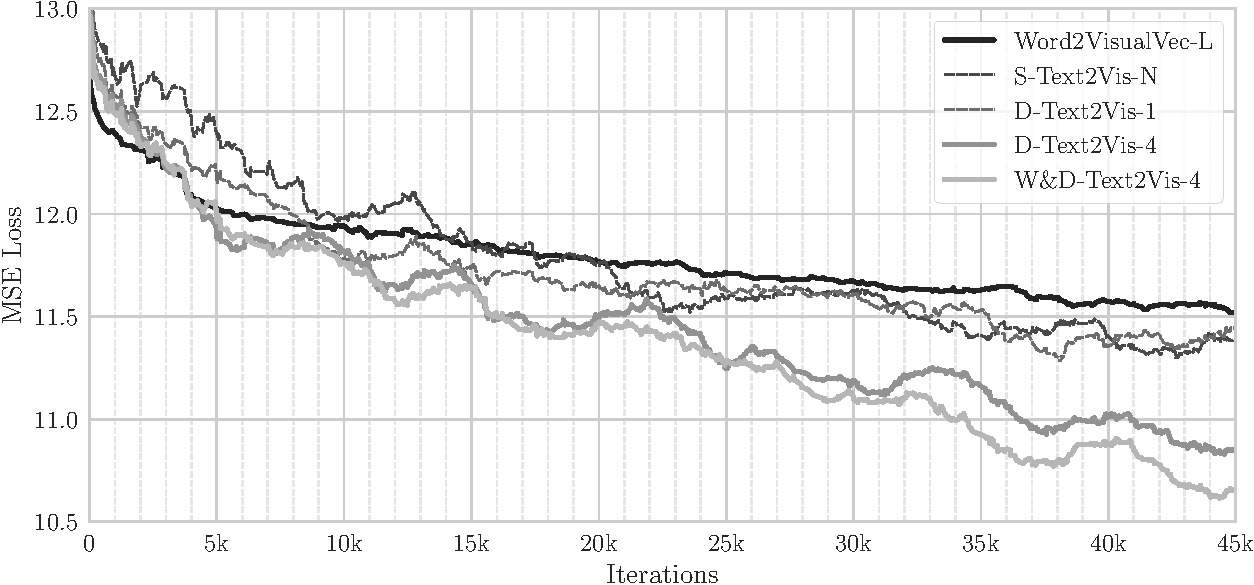
\includegraphics[width=\linewidth]{convergence-plot}
    \caption{Convergence error loss trends on the \emph{fc6} layer of some selected models.}
    \label{fig:t2v:convergence}
\end{figure}


% In addition to the averaged performance, we also investigated how often the ranking produced by \ttv{} is more relevant (according to \gls{dcg}) than those produced by \emph{VisSim} and \emph{VisReg}.
% \ref{fig:t2v:dcgr_dist} indicates that in 69.2\% of the cases, the ranking of \ttv{}$_1$ was found more relevant than \emph{VisSim} (see \ref{fig:t2v:dcgr_dist}).
% The same happens in $58.1\%$ of the cases when comparing \ttv{} to \emph{VisReg}.



% \begin{figure}[ht!]
% \begin{center}
% \includegraphics[width=\textwidth]{text2vis2}
% \end{center}
% \caption{Examples of search results from the three compared methods.}
% \label{fig:t2v:viscomp}
% \end{figure}
%--------------------------------------------------------

%--------------------------------------------------------
% \subsection{Visual comparison}\label{sec:t2v:cases}

% \ref{fig:t2v:viscomp} show a few samples\footnote{More results at \url{https://github.com/AlexMoreo/tensorflow-Tex2Vis}} that highlight the differences in results from the three compared methods.
% In all the cases results from the \emph{VisSim} method are dominated by the main visual features of the images: a face for the first query, the content of the screen for the second query, an outdoor image with a light lower part, plants, people and a bit of sky in the third one.
% The two text based methods obtains results that more often contain the key elements of the description.
% For the first query, \ttv{} retrieves four relevant images out of five, one more that \emph{VisReg}.
% For the other two queries the results are pretty similar, with \ttv{} placing in second position an image that is a perfect match for the query, while \emph{VisReg} places it in fifth position.

%--------------------------------------------------------
\section{Conclusions}
\label{sec:t2v:conclusions}

We have investigated various neural network model designed to learn a projection from a textual space to a visual space, in order to enable cross-media similarity search without reprocessing the representation of the image collection and the relative data structures one may have already produced to perform image similarity search.

The experiments we conducted indicate that our methods produce better results than those produced by performing similarity search directly on the visual features of a query image.
This is an indication that our text-to-image mappings produce better prototypical representations of the desired scene than the representation of a sample image itself.
A simple explanation of this result is that textual descriptions strictly emphasize the relevant aspects of the scene the user has in mind, whereas the visual features, directly extracted from the query image, are keeping track of all the information that is contained in that image, causing the similarity search to be potentially confused by secondary elements of the scene.

Our results also indicate that our methods produce better results than those obtained by similarity search methods on the textual space where the images are indexed by means of automatically generated captions.
%\blue{Despite that being remarkable, there are further incentives in searching in the visual space which refer to the fact that such a space is language-independent.
%As long as our understanding in computational linguistics gets forward, the research community will presumably deliver more and more powerful technologies to produce artificial texts.
%Those technologies might be directly leveraged by our system by means of improved machine translation tools to open the applicability of the text-to-image mapping to multilingual scenarios, without requiring the model to be retrained.
%The same technologies might however become a fundamental part of the caption generation systems, requiring them to retrain the modified models.}
The better results that visual-space based methods have produced over textual-space based ones are not the only argument in favor of the former.
We deem that a stronger argument in favor of visual-space methods is the fact the any improvement to the projection method does not require to reprocess the entire image collection, affecting it only the query processing pipeline.
A web scale image collection can thus immediately benefit from a model update without requiring any processing.
Moreover, a single image similarity search data structure can serve multiple cross-media search models, e.g., built for different languages or specialized on different domains.

We have compared against \wordvisual{}, a recently proposed method that, like ours, uses the visual space as the search space.
In our experimental setup, we improved the performance obtained by the original \wordvisual{}$_{cos}$ by switching from cosine similarity to euclidean similarity that uses \gls{pca} and whitening, following the state of the art in similarity search literature.
The improved \wordvisual{} model obtained among the best results, together with \densettv{} and \widedeepttv{}.
Our \widedeepttv{} model improved over \wordvisual{} by a statistical significant margin.
\widedeepttv{} has more parameters than \wordvisual{} but converges much faster.

%In the future we also plan to compare \ttv{} against the recently proposed \emph{Word2VisualVec} \cite{dong2018predicting} model.
One interesting aspect that proved to be effective in our experiments is the use of a different $\t'$ as a constraint for the hidden representation.
When $\t$ and $\t'$ are different, though semantically similar, the autoencoder branch becomes semantically constrained.
We have investigated this idea in the \sparsettv{}, and we believe the same principle could also bring similar benefits for the \densettv{} and \widedeepttv{} models.
We thus plan to investigate the effects of such ``semantic-autoencoding'' principle by adopting a  \emph{Seq2Seg}~\cite{cho2014learning} architecture, i.e.,  by constraining the final memory state from an encoding \gls{lstm} after processing the input $\t$ to be a good representation to generate a different, but semantically similar, $\t'$ with a decoder \gls{lstm}.
We believe such an intermediate state to be able to produce better projections to the visual features.

